\documentclass{article}

\usepackage[utf8]{inputenc}
\usepackage[T1]{fontenc}
\usepackage[francais]{babel}
\usepackage{url}
\usepackage{color}
\usepackage{verbatim}
\usepackage{amsmath,amssymb,amsfonts}
\usepackage{graphicx}
\usepackage[french]{algorithm2e}
\usepackage{geometry}
\usepackage{caption}
\captionsetup[figure]{slc=on}
\usepackage{enumitem}
\usepackage{listings}
\usepackage{listingsutf8}
\frenchbsetup{StandardLists=true}
\usepackage{mcode}
\lstset{language=matlab}
\lstset{
	breaklines=true, 
	showspaces=false, 
	keepspaces=true, 
	numbers=left, 
	frame=shadowbox, 
	keywordstyle=\color{blue},
	basicstyle=\ttfamily\small,
	commentstyle=\color{green}
}
\geometry{hmargin=2.5cm, vmargin=2.5cm}

\title{\textbf{Traitement d'images TP4 : Détection de contour}}
\author{Line \bsc{POUVARET}, Hamdi \bsc{BENAOUN}}
\date{2015-2016}

\begin{document}
\maketitle

\section*{2. Dérivation par simples différences finies}
\subsection*{2.1 Filtre de Roberts}
\begin{itemize}\renewcommand{\labelitemi}{$\bullet$}
	\item Fonction roberts\_differential, dans MatLab :
	
\begin{lstlisting}
pic_x = conv2(pic, D, 'same');
pic_y = conv2(pic, D', 'same');
\end{lstlisting}

	\item calcul de la norme, dans MatLab :
\begin{lstlisting}
pic_norm = sqrt(power(pic_x, 2)+power(pic_y, 2));
\end{lstlisting}
	\item Images des gradients en x, y et de la norme :
	
\fbox{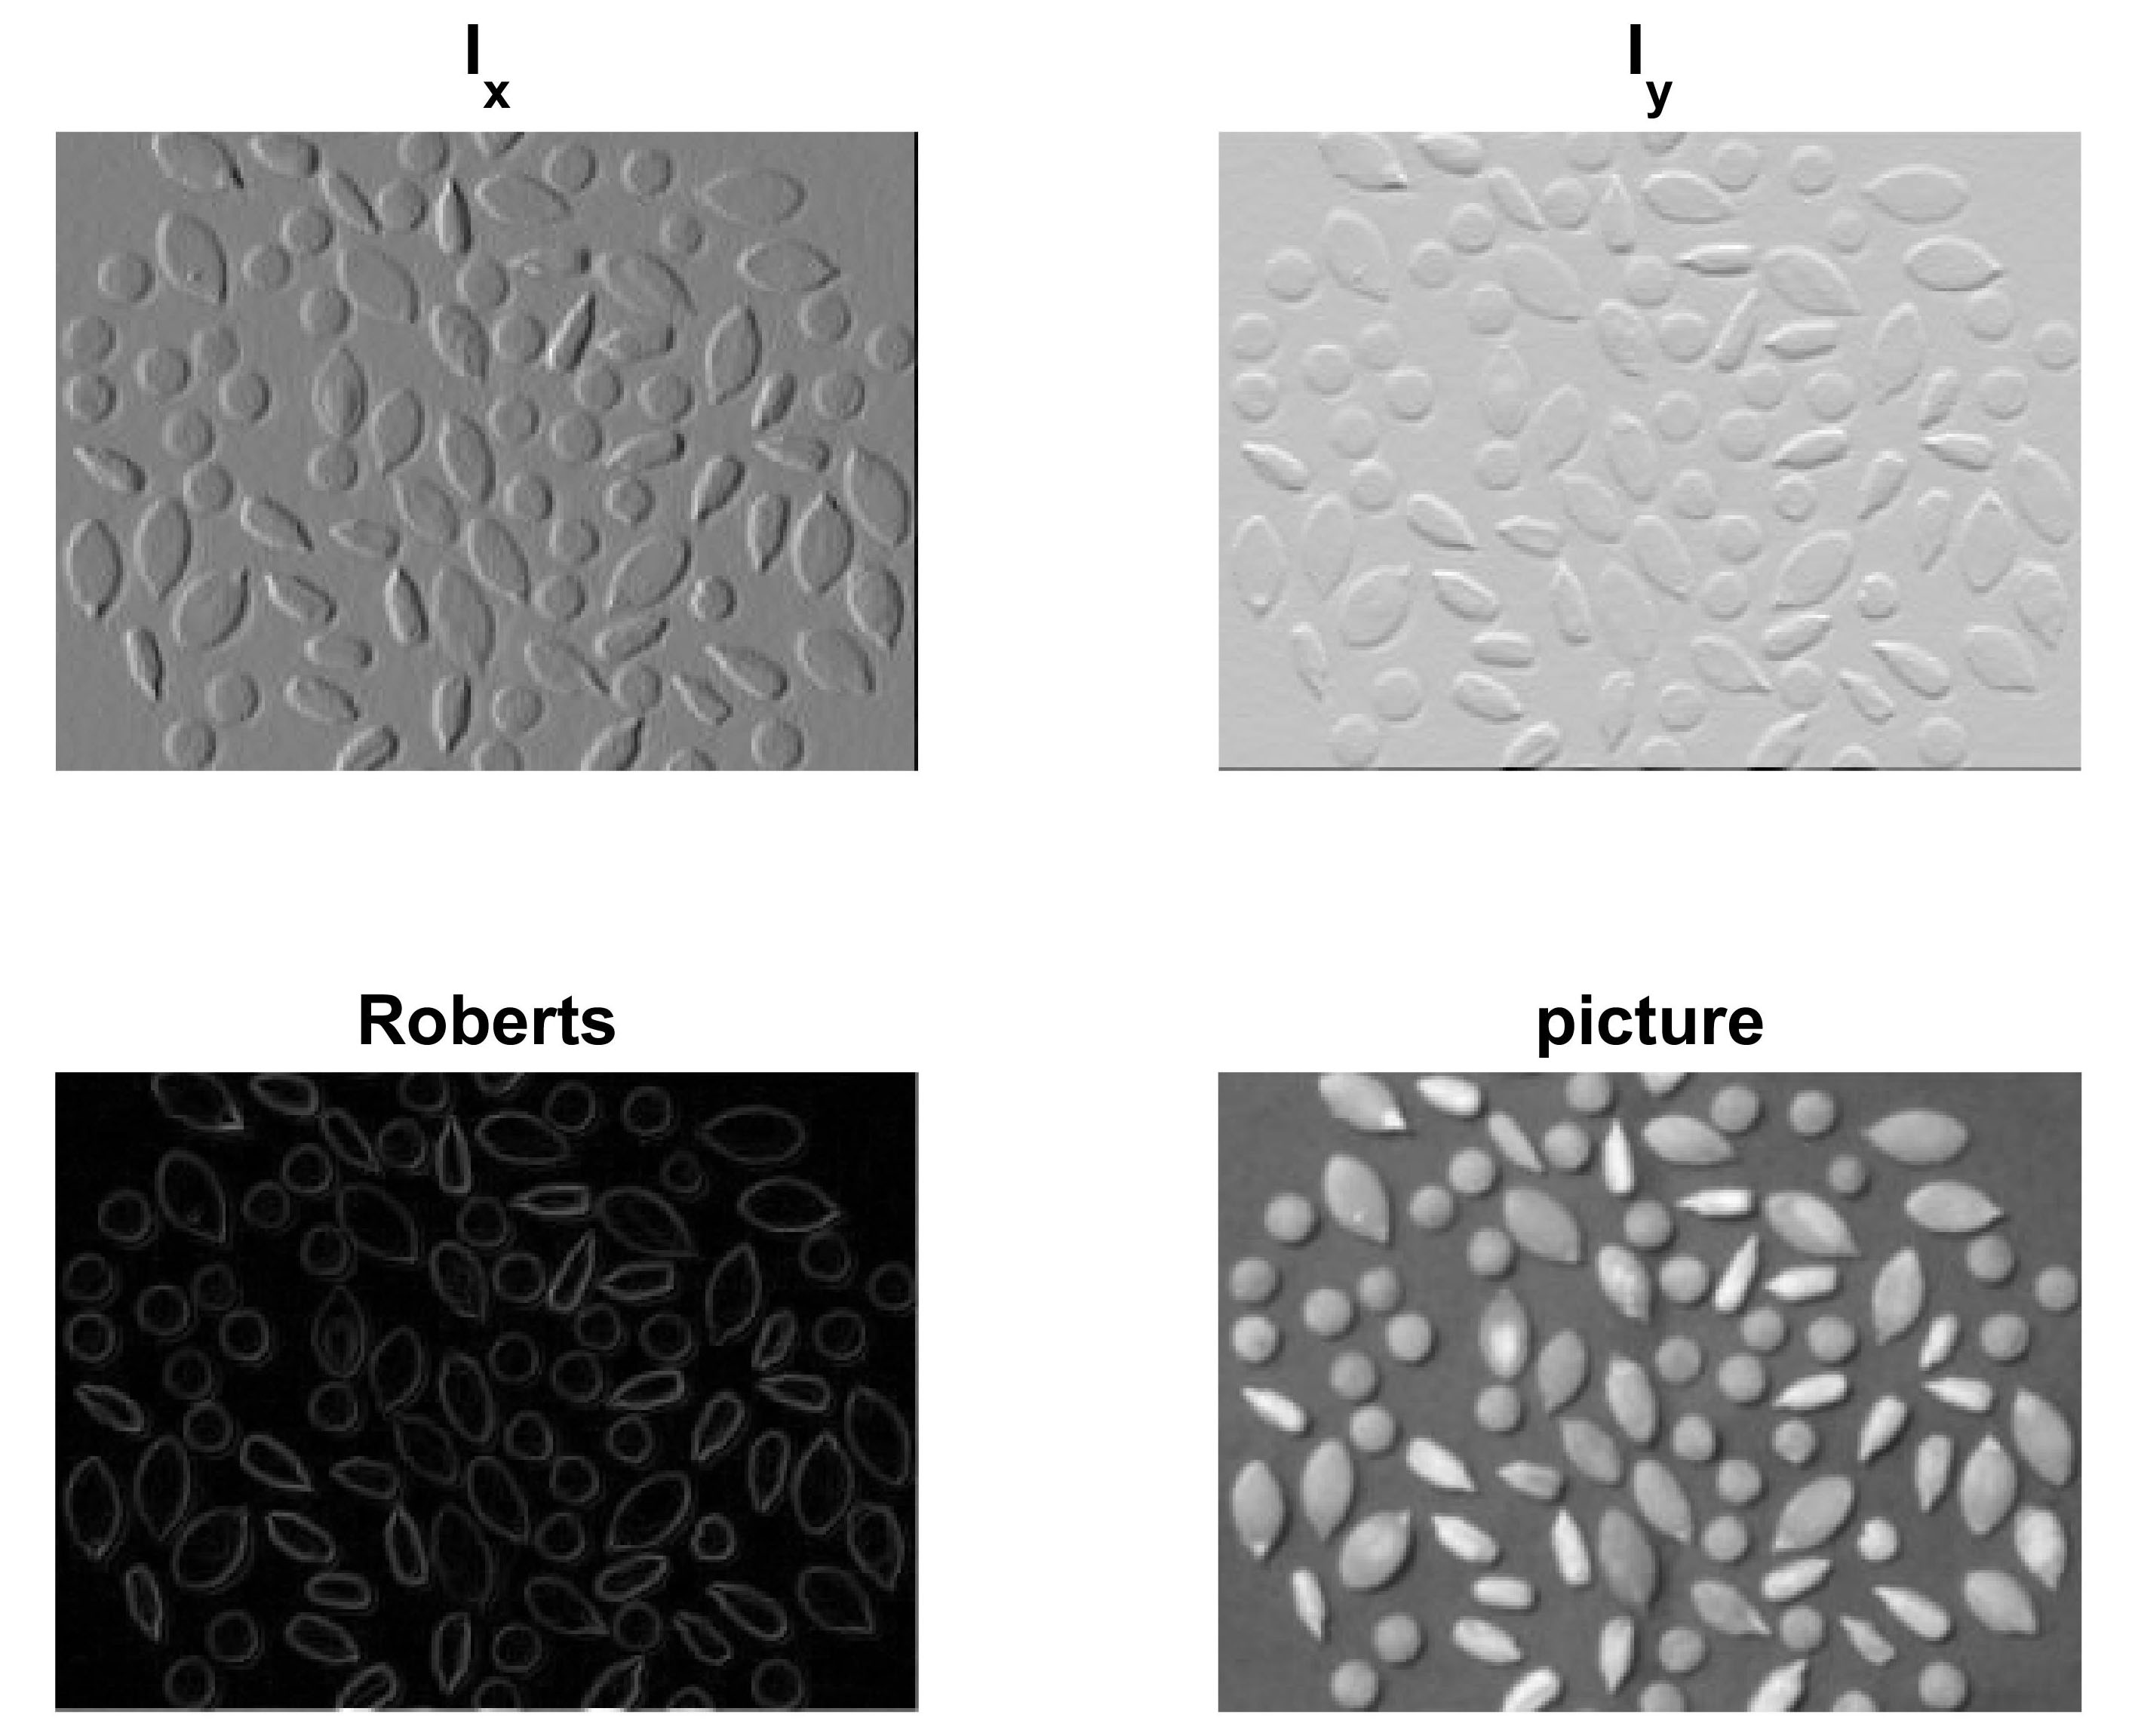
\includegraphics[width=15cm]{gradients_norme_graines.jpg}}

On remarque au niveau de l'image de la norme, que certaines ombres des graines sont détectés comme des contours (c'est logique puisqu'il y a une variation du sombre au clair).

\end{itemize}

\subsection*{2.2 Filtre de Sobel}

\begin{itemize}\renewcommand{\labelitemi}{$\bullet$}
	\item Fonction sobel\_differential dans MatLab :
	
\begin{lstlisting}
S=[1,2,1];
D=[1,0,-1];
Gx=S'*D;
Gy=D'*S;

pic_x = conv2(pic, (1/4)*Gx,'same');
pic_y = conv2(pic, (1/4)*Gy, 'same');

pic_norm = sqrt(power(pic_x, 2)+power(pic_y, 2));
\end{lstlisting}

	\item Images des gradients en x, y et de la norme :
	
\fbox{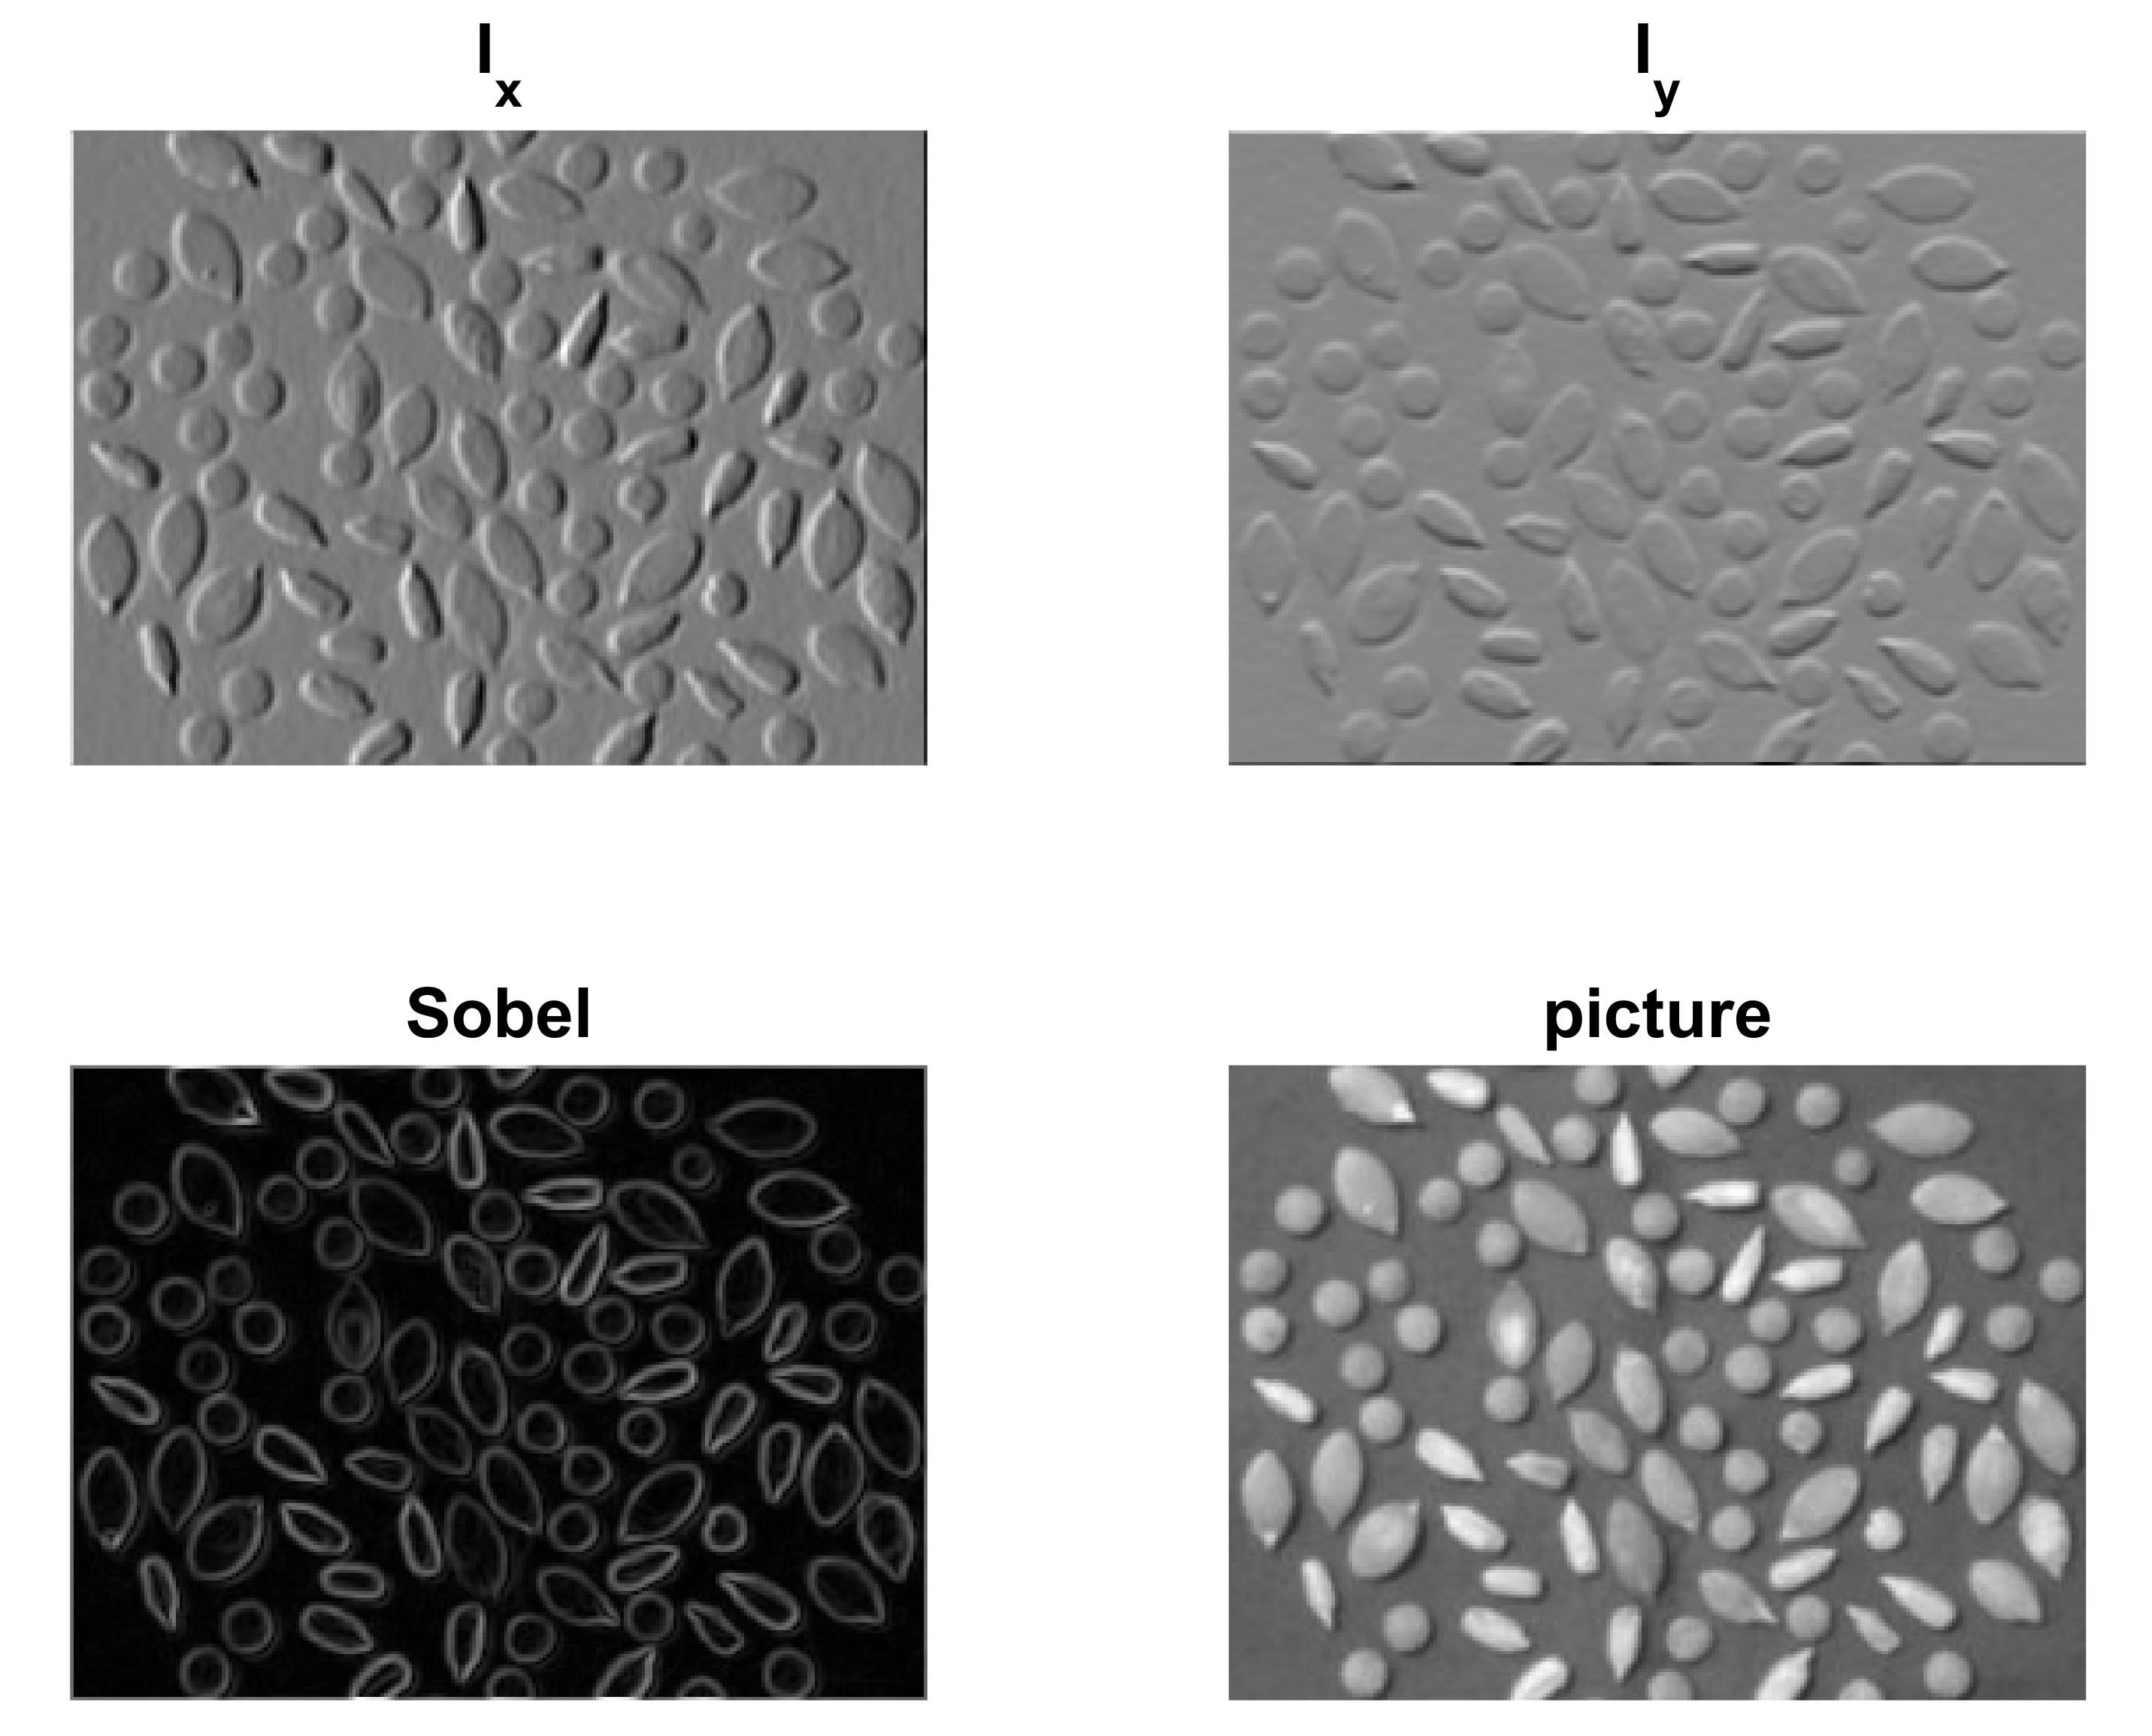
\includegraphics[width=15cm]{gradients_norme_sobel.jpg}}

Les vrais contours des graines sont beaucoup plus nets. On constate tout de même encore un peu les ombres qui ont été détectées mais elles sont beaucoup moins visibles.
\end{itemize}

\subsection*{2.3 Ajout d'un bruit gaussien}
On ajoute un bruit gaussien avec RSB = 10db.
\begin{itemize}\renewcommand{\labelitemi}{$\bullet$}
	\item Avec le filtre de Roberts :
	
\fbox{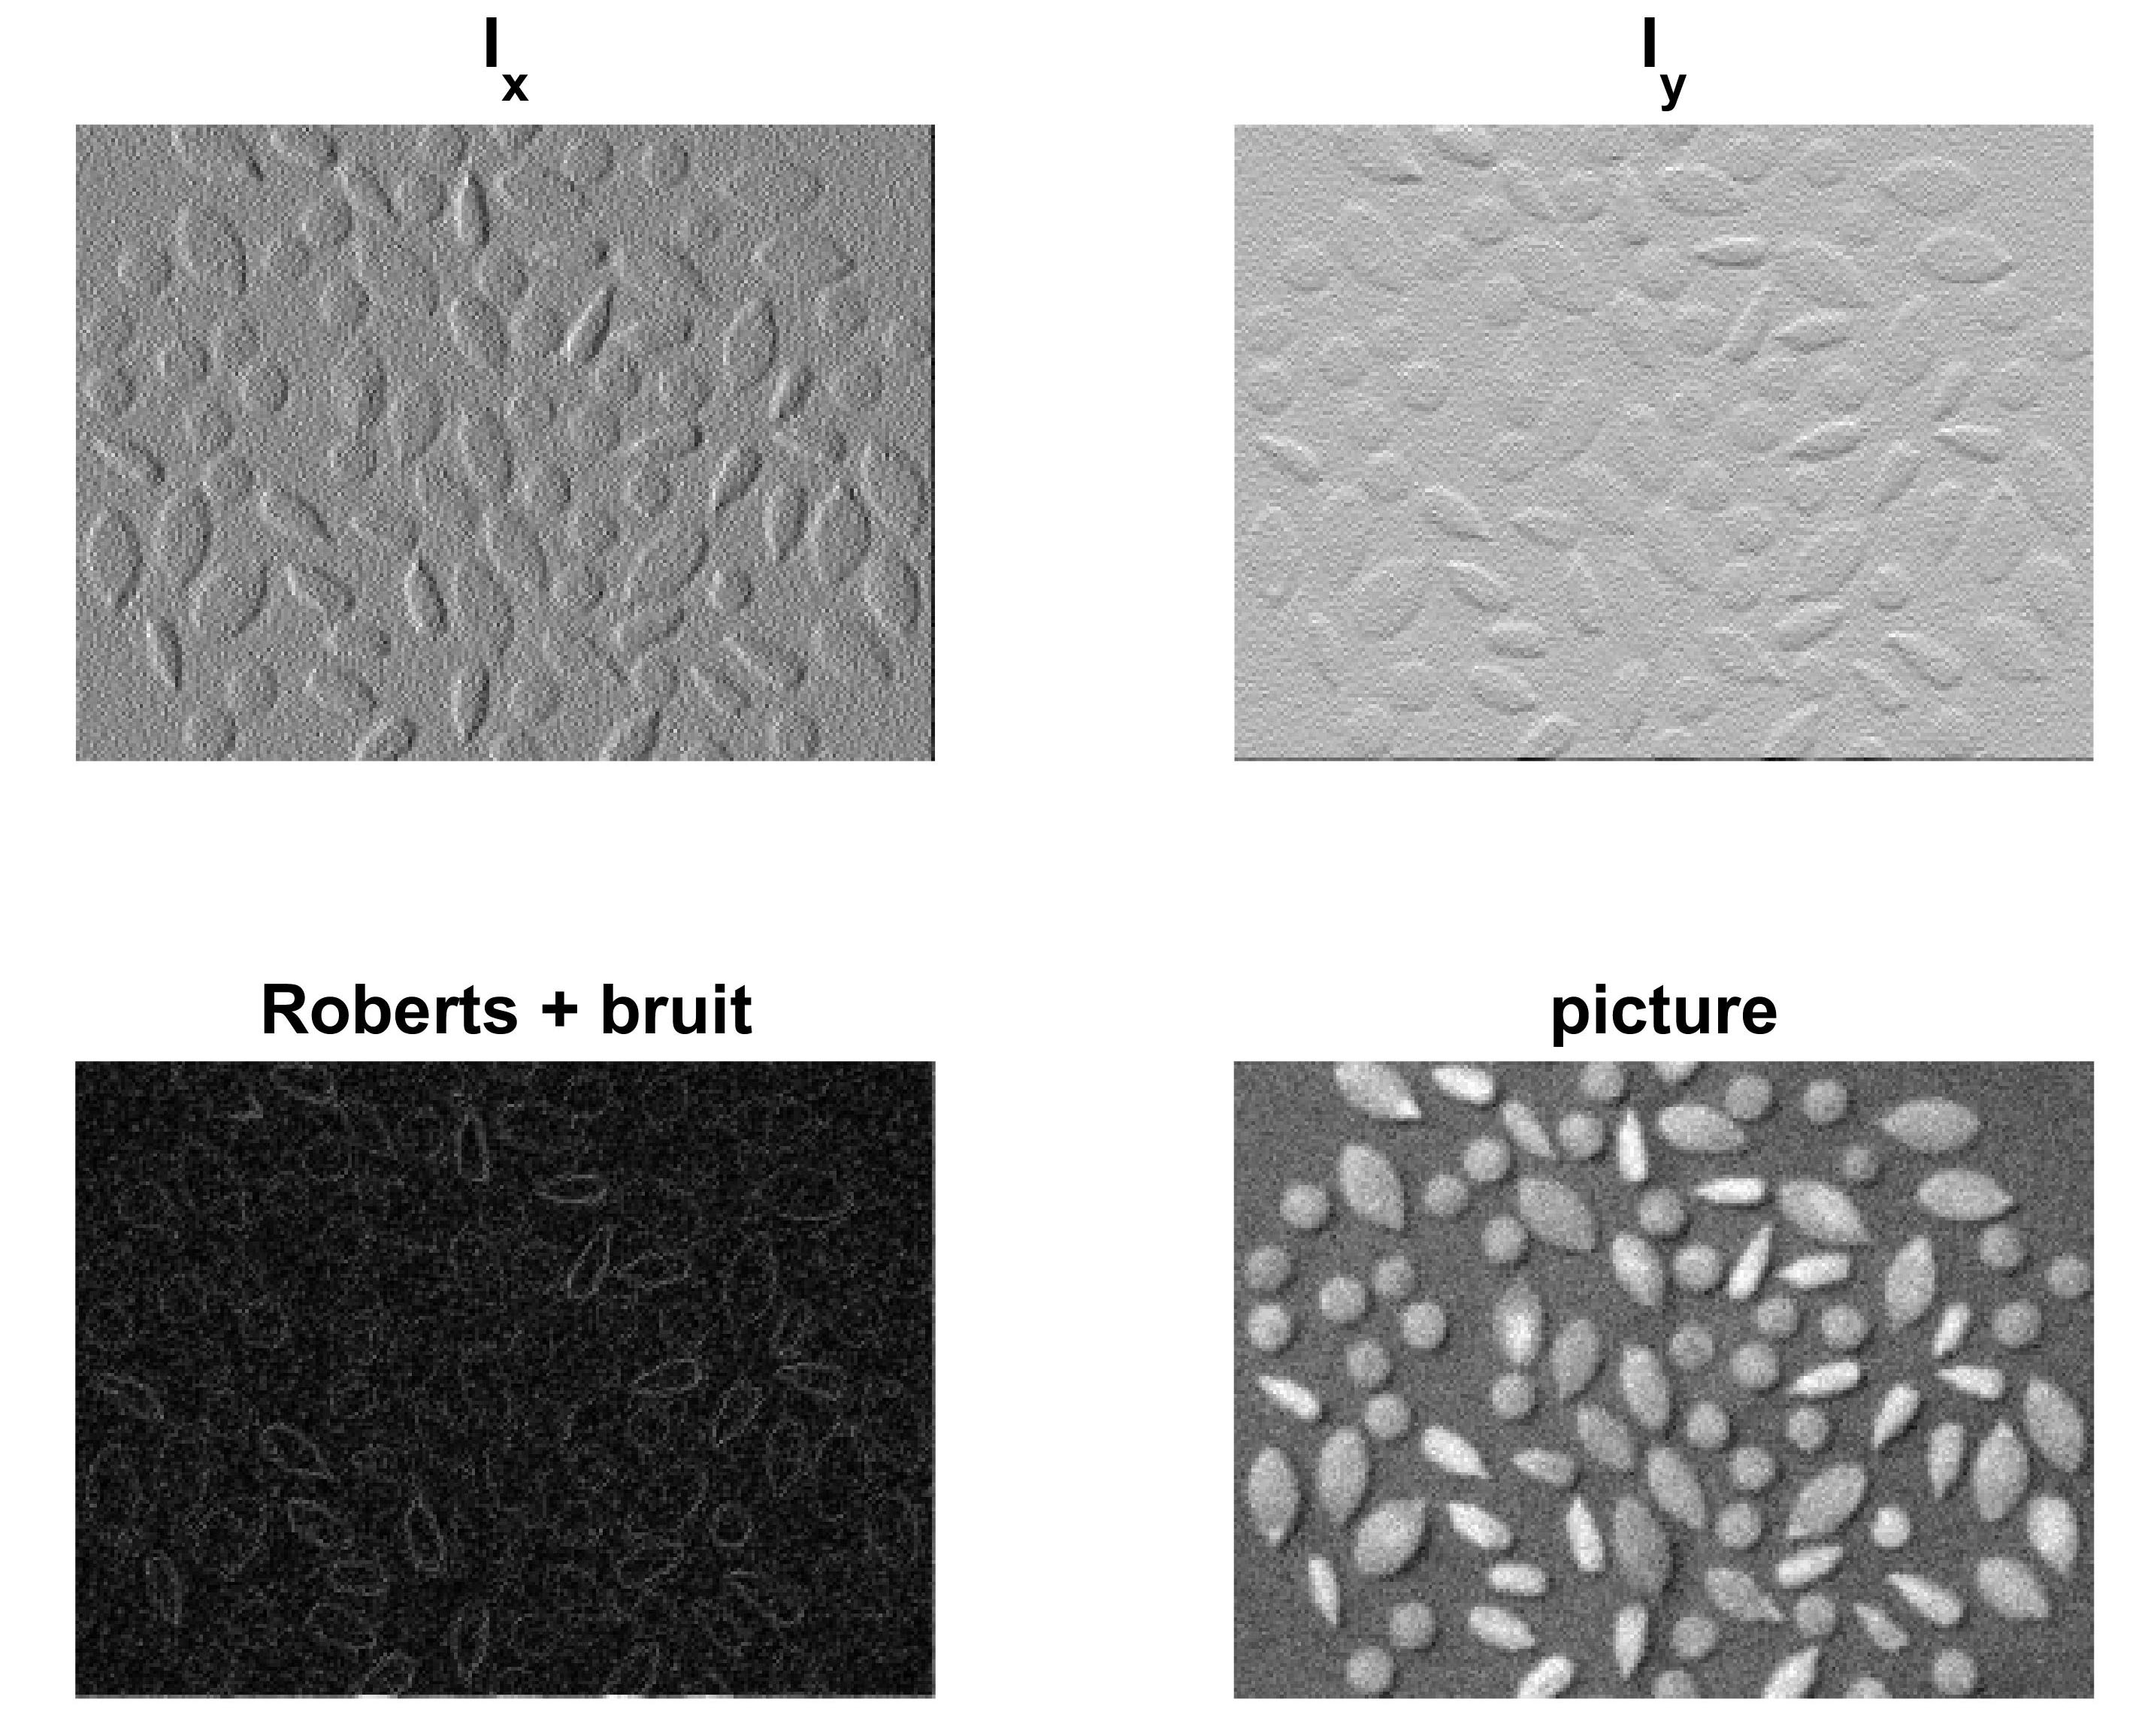
\includegraphics[width=15cm]{bruit_gauss_roberts.jpg}}
	\item Avec le filtre de Sobel :
	
\fbox{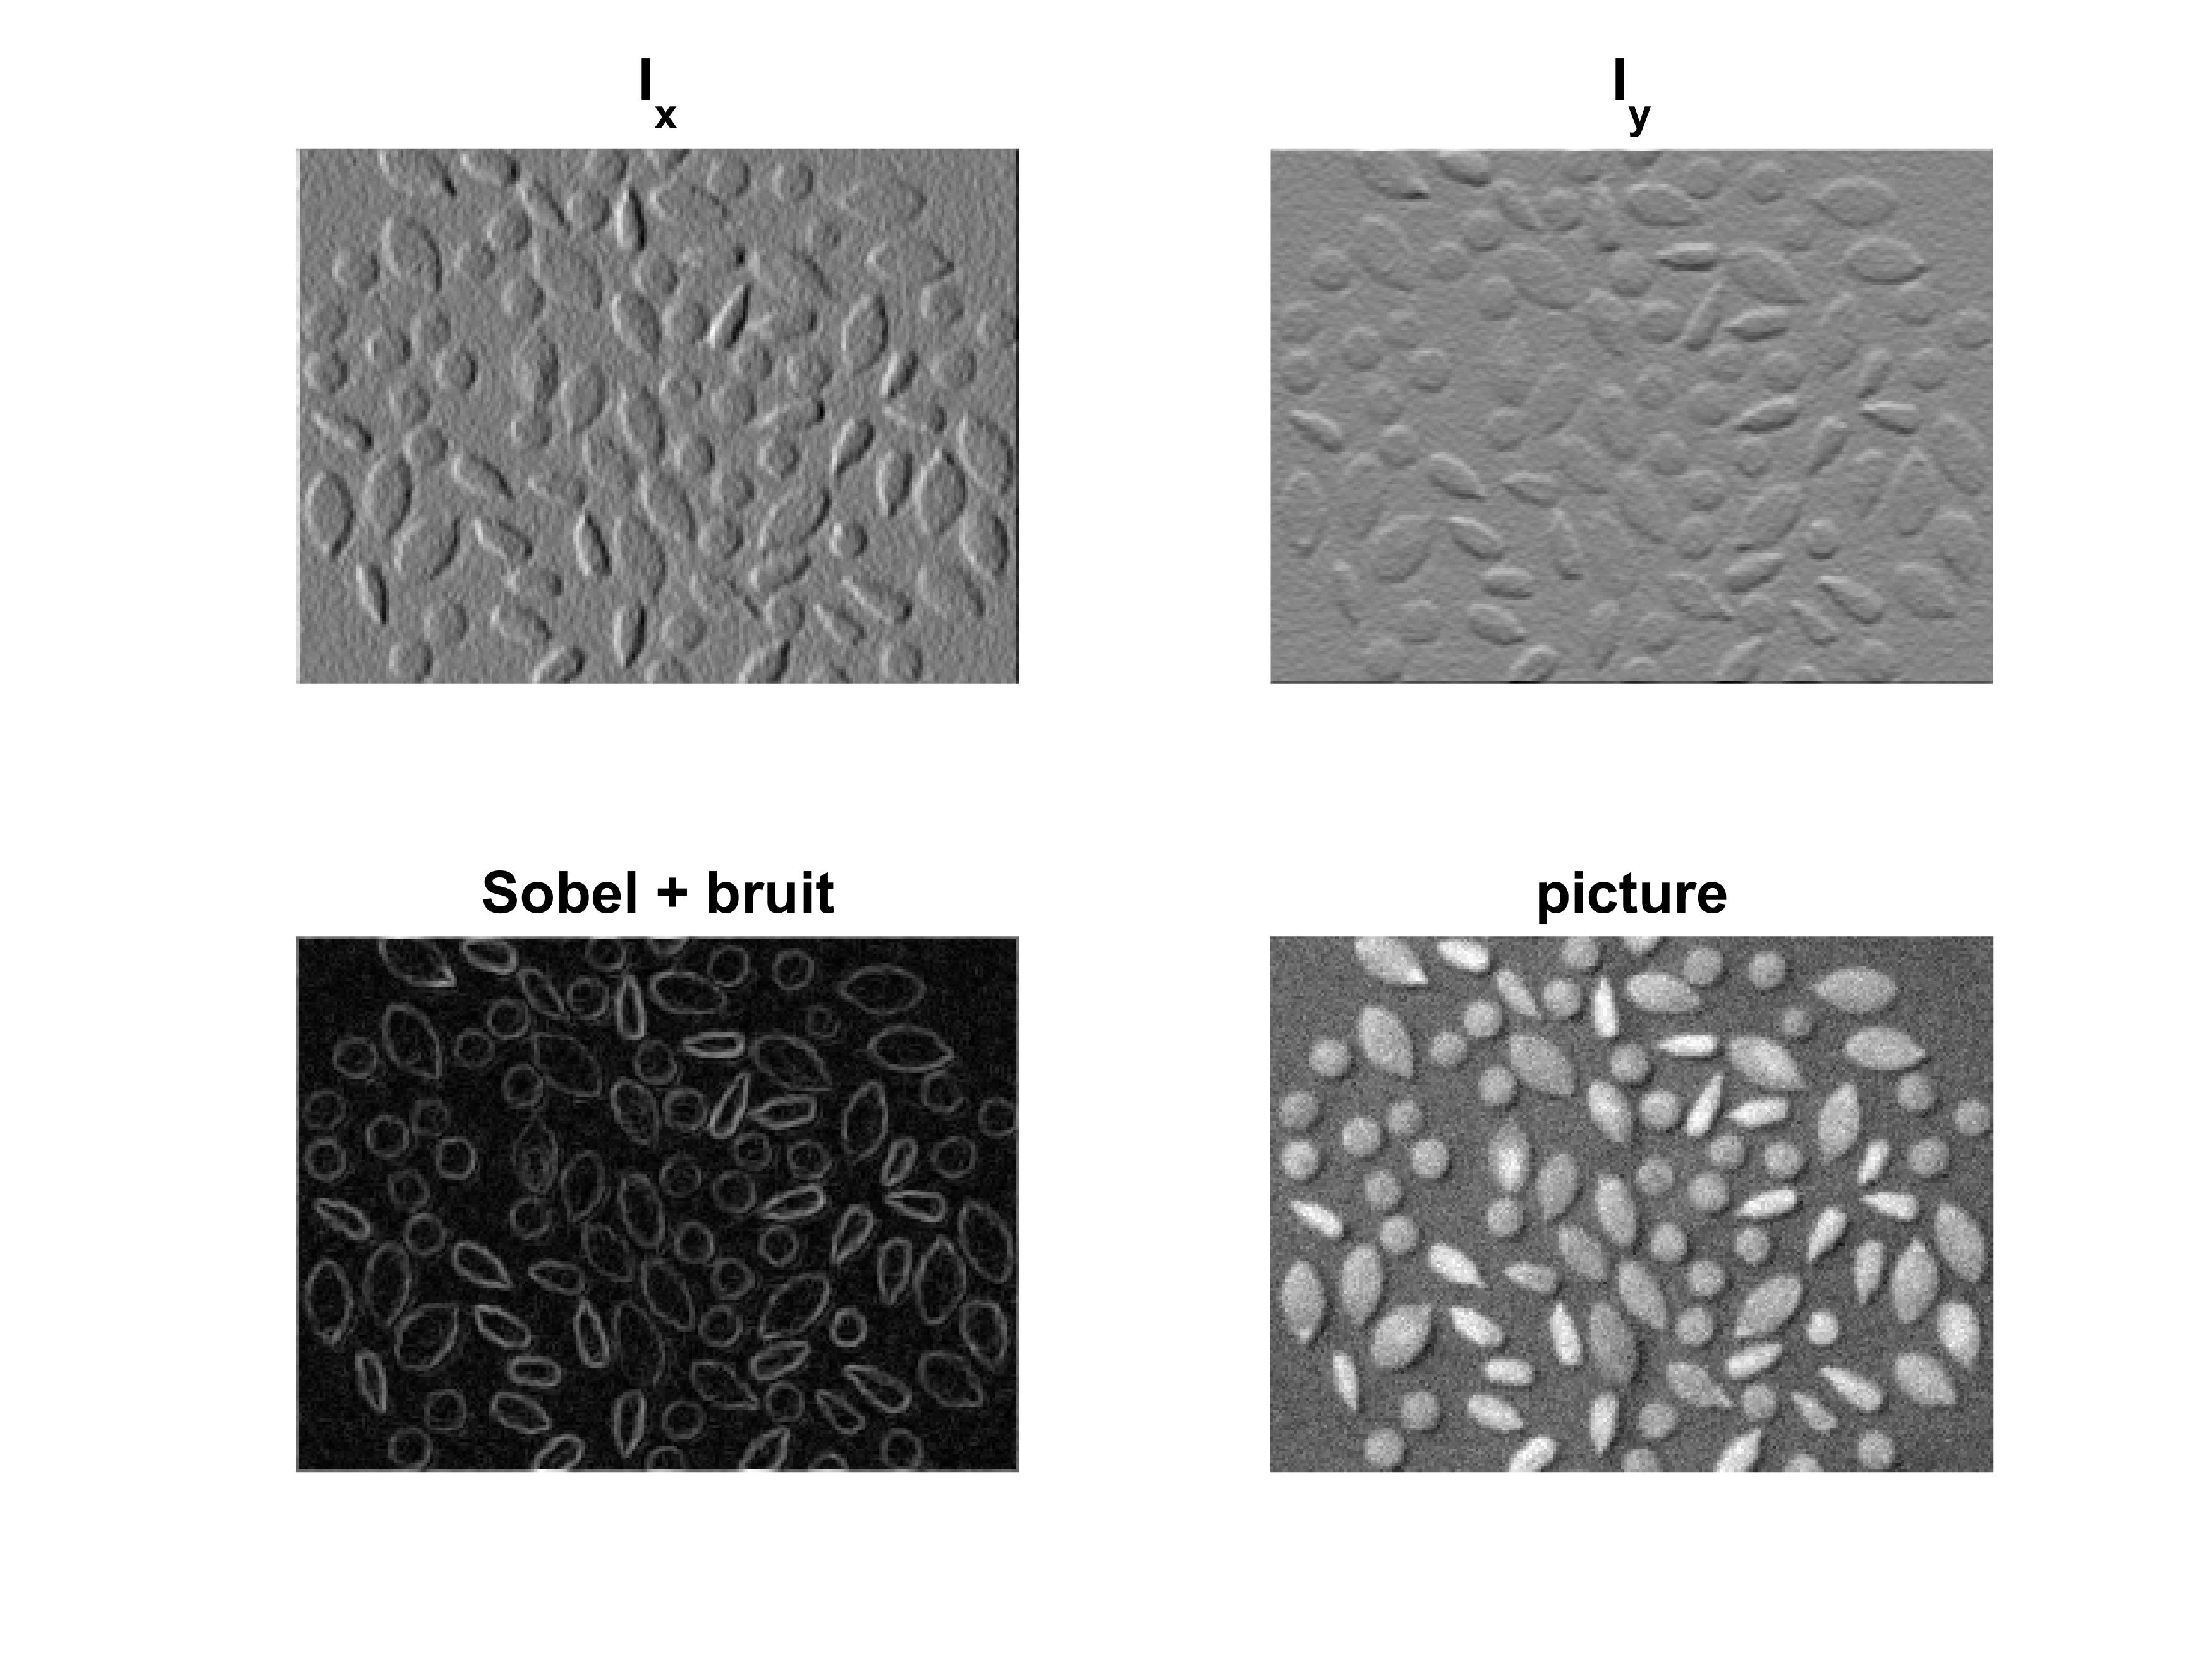
\includegraphics[width=15cm]{bruit_gauss_sobel.jpg}}	
\end{itemize}

On constate que la méthode utilisant le filtre de Roberts n'est vraiment pas efficace dès qu'on a du bruit sur l'image.

En effet, on a du mal à constater correctement les contours des graines.\\

La méthode utilisant le filtre de Sobel est beaucoup plus robuste face au bruit car les contours des graines est assez bien conservé même si on observe légèrement les contours correspondant au bruit dans l'image de la norme.

\section*{3. Recherche des maxima locaux dans la direction du gradient}

\begin{itemize}\renewcommand{\labelitemi}{$\bullet$}
	\item Interpolation au plus proche voisin (nearest)
	
\fbox{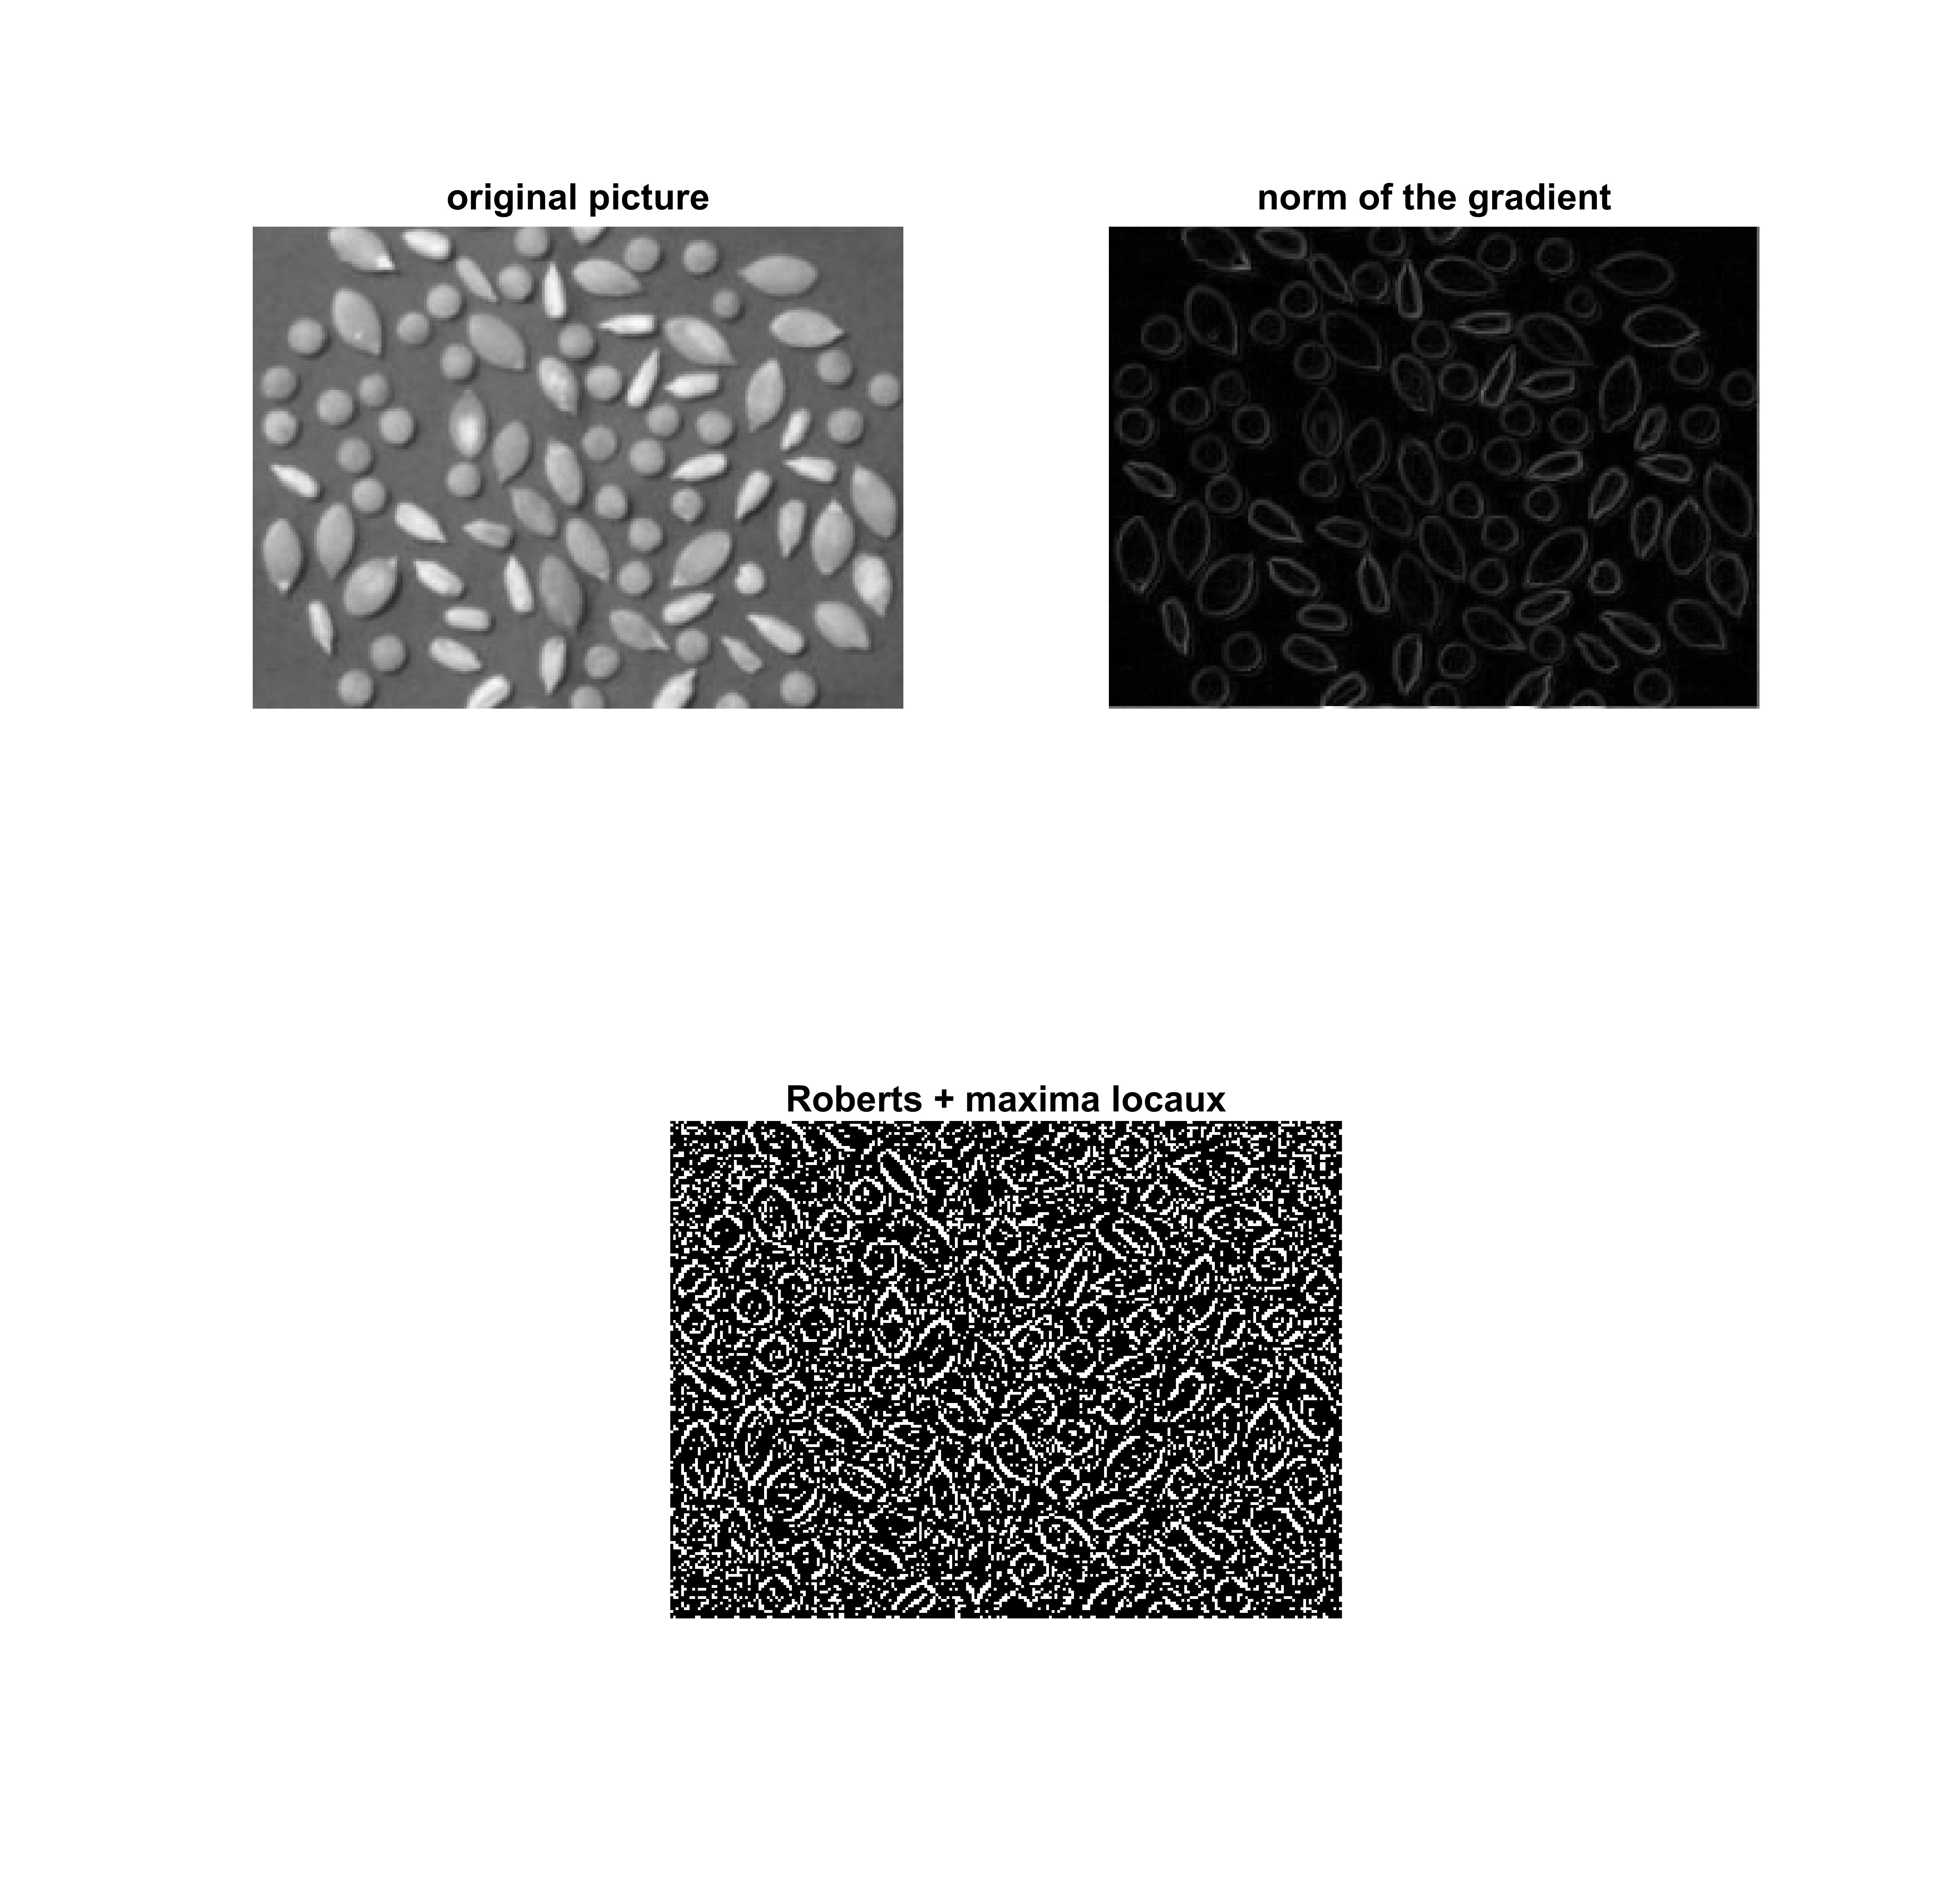
\includegraphics[width=15cm]{roberts_nearest.jpg}}
	
\fbox{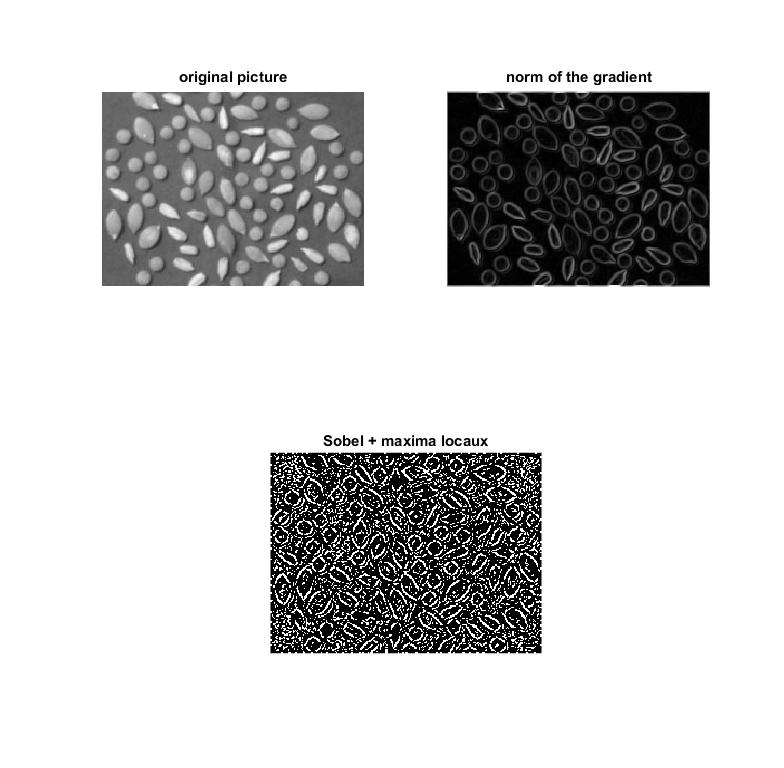
\includegraphics[width=15cm]{sobel_nearest.jpg}}	

	\item Interpolation bilinéaire
	
\fbox{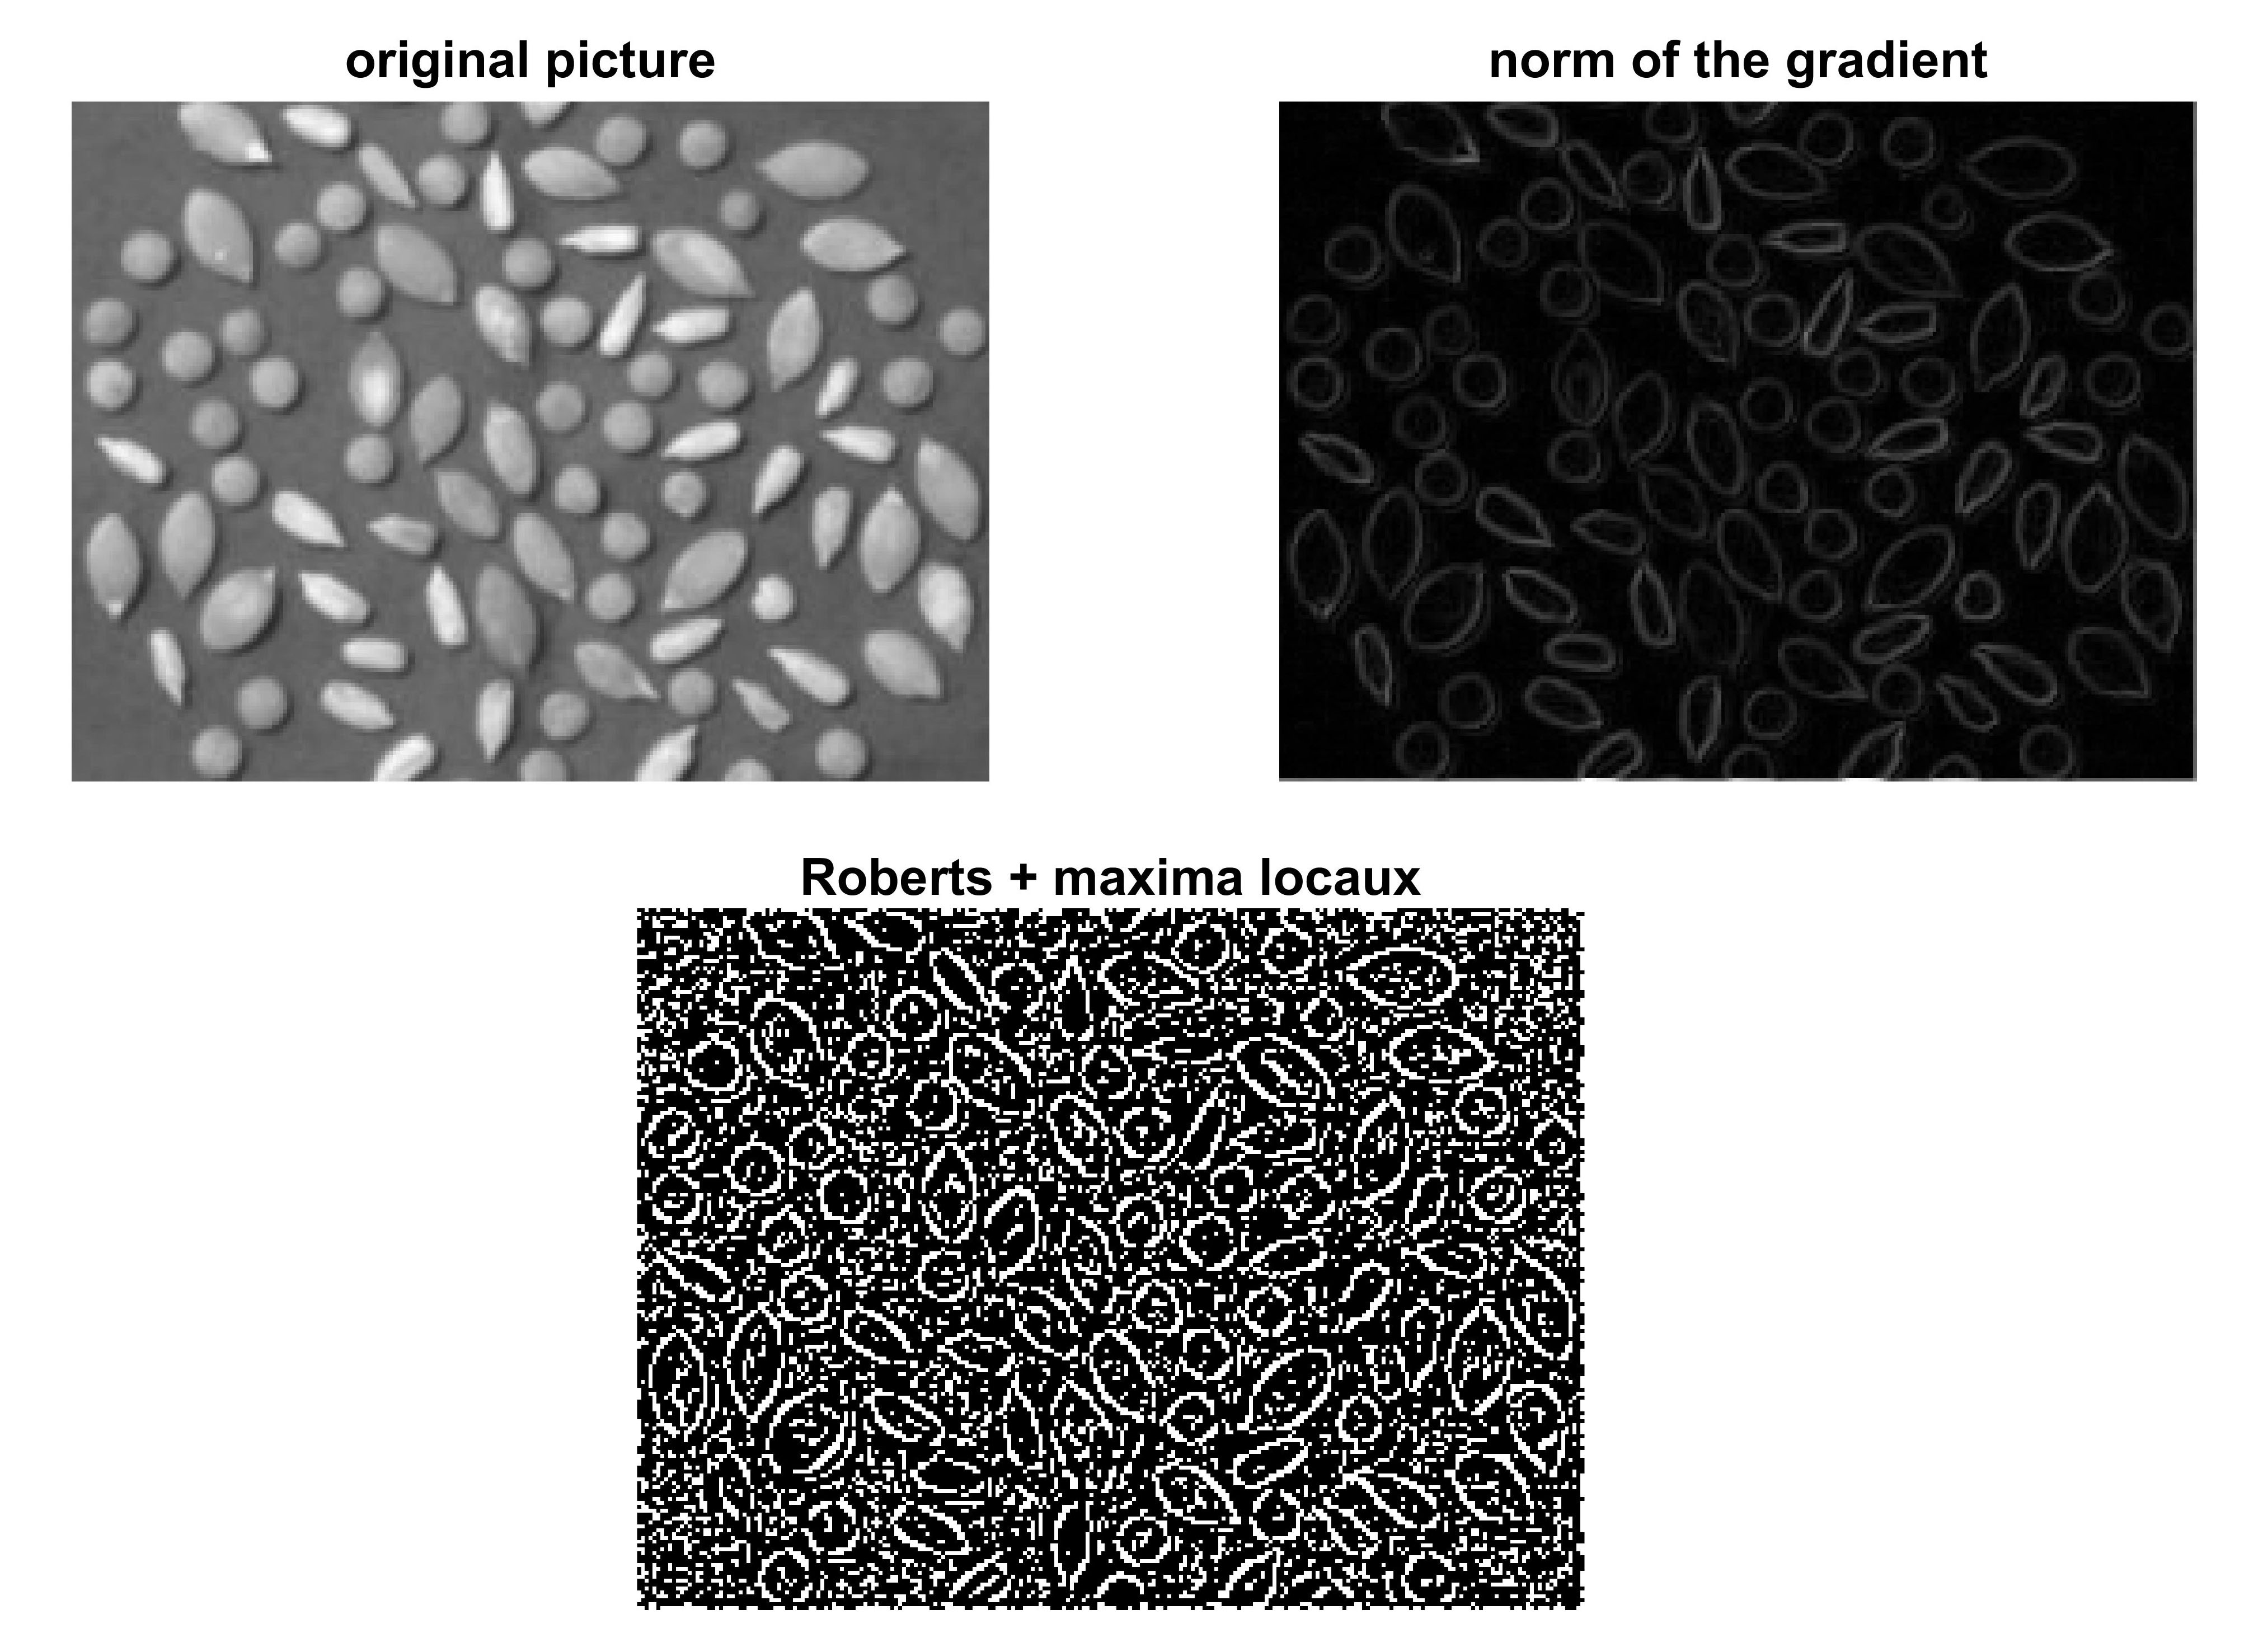
\includegraphics[width=15cm]{roberts_bilinear.jpg}}
	
\fbox{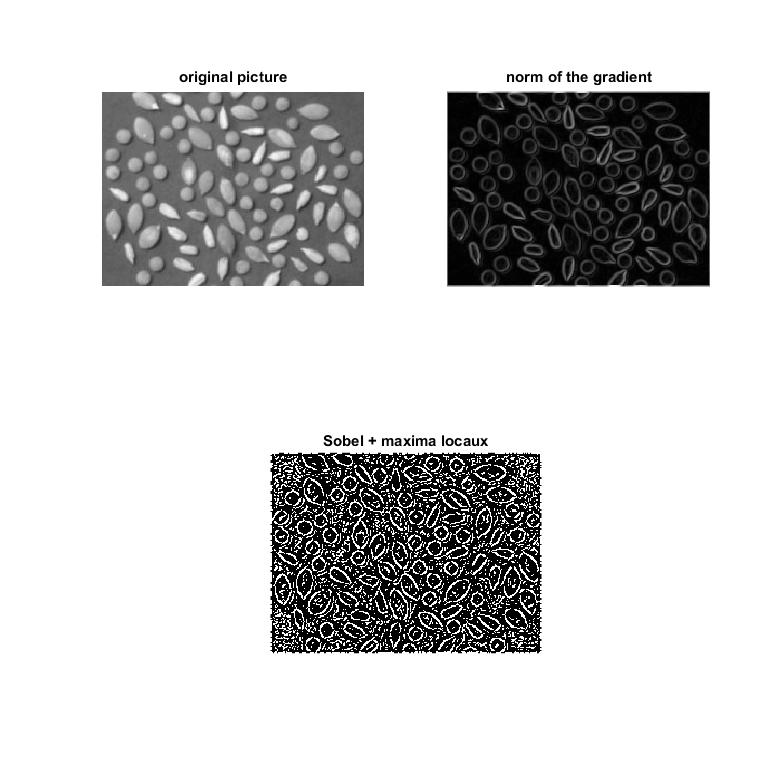
\includegraphics[width=15cm]{sobel_bilinear.jpg}}	

	
\begin{lstlisting}

\end{lstlisting}

\end{itemize}

\section*{4. Seuillage et chaînage des points de contour}

\begin{itemize}\renewcommand{\labelitemi}{$\bullet$}
	\item
	
\begin{lstlisting}

\end{lstlisting}

\end{itemize}

\section*{5. Exécution de la chaîne complète de détection de contours}

\begin{itemize}\renewcommand{\labelitemi}{$\bullet$}
	\item
	
\begin{lstlisting}

\end{lstlisting}

\end{itemize}

\end{document}